\titre{9}
\theme{trigo}
\auteur{Nathan Scheinmann}
\niveau{1M}
\source{sesamath-1M-trigo}
\type{serie}
\piments{2}
\pts{}
\annee{2425}

\contenu{
	\tcblower
	Charlotte navigue le long d'une falaise. Pour des questions de sécurité, elle ne doit pas aller au delà du point $C$. Elle a jeté l'ancre au point $B$. On a $\overline{SH}=100~\text{m}, \widehat{HCS}=75^\circ$ et $\widehat{HBS}=65^\circ$. 
	\begin{center}
	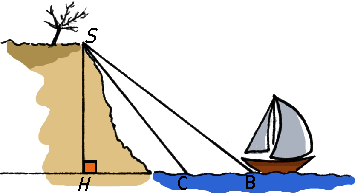
\includegraphics[scale=1]{../medias/1M/trigo/1M-exo-9}
	\end{center}
	À quelle distance du point $C$ le bateau de Charlotte se trouve-t-il~? Doner la valeur approchée au mètre près.
}
\correction{

}

